\documentclass[11pt,spanish,a4paper]{article}
% Versión 1er cuat 2014 Víctor Bettachini < bettachini@df.uba.ar >

\usepackage{babel}
\addto\shorthandsspanish{\spanishdeactivate{~<>}}
\usepackage[utf8]{inputenc}
\usepackage{float}
\usepackage{units}
\usepackage{siunitx}
\usepackage{amsmath}
\usepackage{amstext}
\usepackage{amssymb}
\usepackage{graphicx}
\graphicspath{ {./graphs/} {../}}

\voffset-3.5cm
\hoffset-3cm
\setlength{\textwidth}{17.5cm}
\setlength{\textheight}{27cm}

\usepackage{lastpage}
\usepackage{fancyhdr}
\pagestyle{fancyplain}
\fancyhead{}
\fancyfoot{}
\fancyfoot[C]{ {\tiny Actualizado al \today} }
\fancyfoot[RO, LE]{Pág. \thepage/\pageref{LastPage}}
\renewcommand{\headrulewidth}{0pt}
\renewcommand{\footrulewidth}{0pt}


\begin{document}
\begin{center}
	\textsc{\large Física 2 (Físicos)} - Prof. Hernán Grecco\\
	\textsc{\large Primer Cuatrimestre - 2014}\\
	\textsc{\large Guía 2:} Sistemas con más grados de libertad
\end{center}

\begin{enumerate}
\item
\begin{enumerate}
	\item Considere el sistema de la figura en ausencia de gravedad y obtenga sus frecuencias naturales de oscilación y los modos normales
	correspondientes.
	Escriba las ecuaciones de movimiento de cada masa.
	\item Sabiendo que en \(t=0\) el sistema satisface las siguientes condiciones \(\Psi_a(0)=1\) y \(\Psi_b(0)=0\) y que se encuentra en reposo, encuentre el movimiento de cada partícula.
	\item Analice cómo se modifica el resultado por la presencia de la gravedad.
	\end{enumerate}
 	\begin{center}
		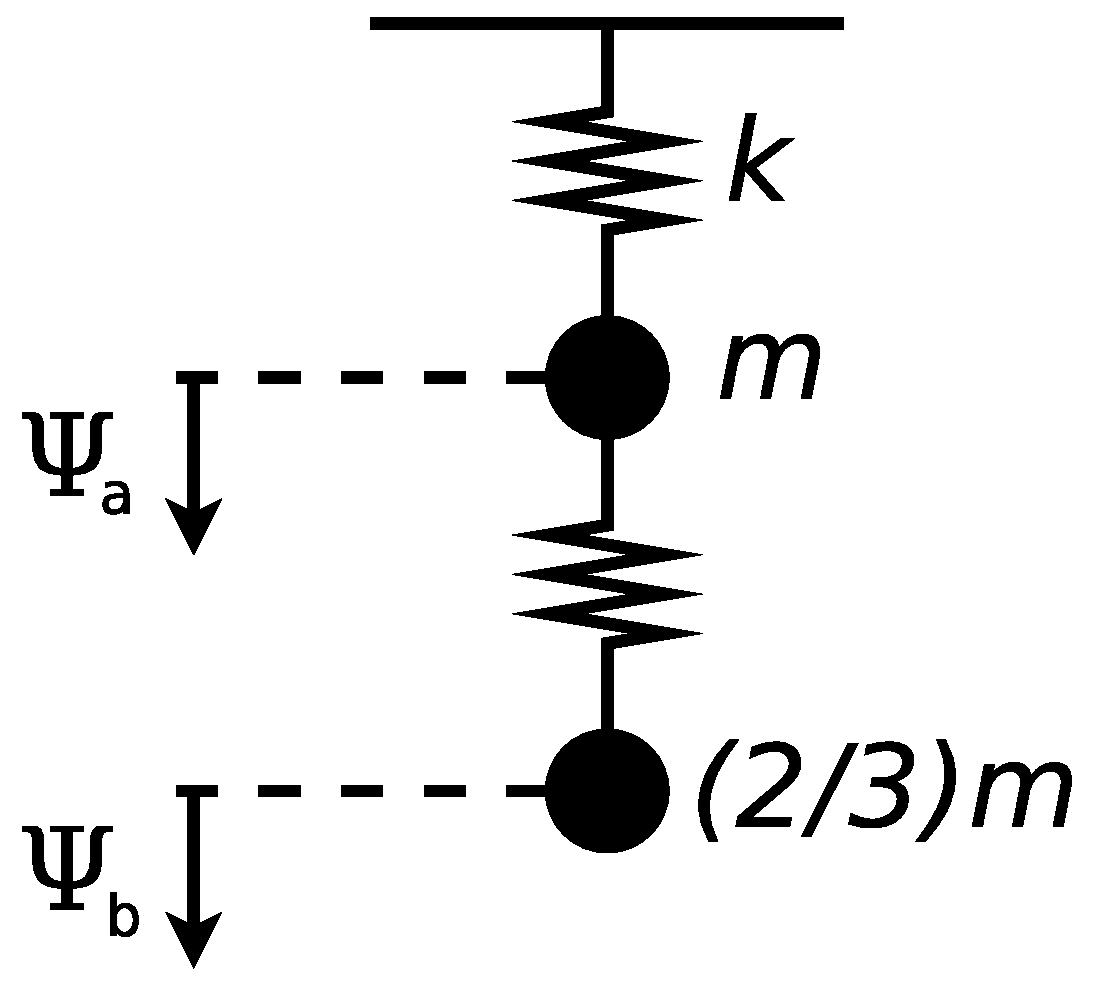
\includegraphics[width=0.2\linewidth]{ej1-6}
 	\end{center}

\item
	Considere el sistema de la figura.
	Las masas están apoyadas en una mesa sin rozamiento, sujetas a las paredes por resortes de constante \(k\) y unidas por otro resorte de constante \(k'\).
	Obtenga las frecuencias y los modos transversales del sistema.
	¿Bajo qué condiciones espera observar batidos?
	¿Qué son batidos?

    \begin{center}
		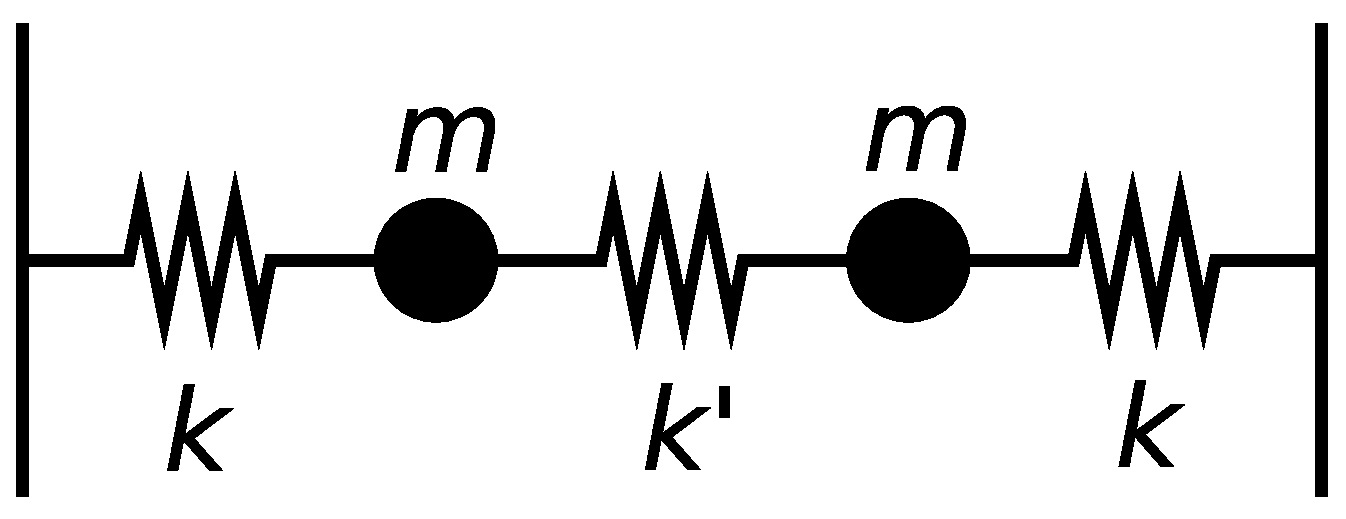
\includegraphics[width=0.2\linewidth]{ej1-8}
    \end{center}

\item
	Considere el sistema simplificado de la figura que se basa en una molécula triatómica simétrica.
	En el equilibrio dos átomos de masa m están situados a ambos lados del átomo de masa \(M=2m\) y vinculados por resortes de constante \(k\) y longitud natural \(l_o\).
	Como sólo estamos interesados en analizar los modos longitudinales.
	\begin{enumerate}
		\item Encuentre las ecuaciones de movimiento de cada masa.
		\item Halle las frecuencias de los modos normales.
		\item Dibuje las configuraciones de cada modo.
		\item Si el centro de masa de la molécula se mueve con \(v_o=\mathrm{cte}\), halle la solución para \(\Psi_a(t)\), \(\Psi_b(t)\) y \(\Psi_c(t)\).
		\item Establezca cuáles deben ser las condiciones iniciales para excitar sólo el modo más alto (mayor frecuencia).
		\item Si se aplica a una de las masas una fuerza armónica, ¿a cuál conviene aplicarla para excitar más eficientemente el modo de mayor frecuencia?
	\end{enumerate}
	\begin{center}
	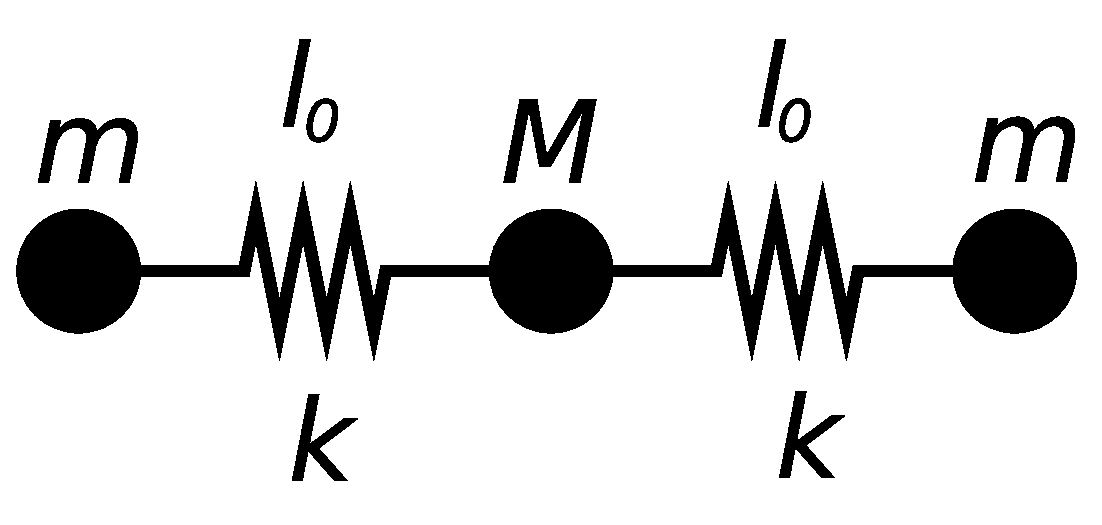
\includegraphics[width=0.2\linewidth]{ej1-9}
	\end{center}


\item Se analizan las oscilaciones transversales del sistema de la figura.
	\begin{enumerate}
		\item Encuentre las ecuaciones de movimiento de las masas.
		\item Halle las frecuencias de los modos normales.
		\item Dibuje la configuración correspondiente a cada modo normal.
		\item Si el centro de masa se encuentra en reposo, determine los desplazamientos de cada masa como función del tiempo.
		\item ¿Qué condiciones iniciales que permiten excitar sólo el segundo modo?
		\item Si se fuerza la masa del centro y se va variando la frecuencia, ¿qué modos se observan?
		\item ¿Cómo se modifican los resultados anteriores si el extremo de la derecha se fija a la pared?
	\end{enumerate}
	\begin{center}
		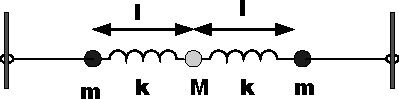
\includegraphics[width=0.4\linewidth]{g02e04}
	\end{center}

\item Denominamos a los ángulos en que se aparta cada barra del equilibrio \(\alpha_1\), \(\alpha_2\) y \(\alpha_3\).
	Uno de los modos de oscilación del sistema será cuando oscila como péndulo rígido.
	Para este caso las tres coordenadas son iguales y el vector posición será \((\alpha_1, \alpha_2, \alpha_3)= \alpha (1,1,1) \).
	Este es el modo en que oscila el centro de gravedad del conjunto.
	Otro modo es cuando un extremo oscila para un lado, el centro queda quieto y el otro extremo se mueve en sentido contrario: \((\alpha_1, \alpha_2, \alpha_3)= \alpha (1,0,-1)\).
	En este caso el centro de gravedad no se mueve.
	Por la simetría del problema (tres barras iguales) el tercer caso resulta de pensar cual es el movimiento de los tres cuerpos que queda que deja quieto en centro de gravedad, y es el del centro hacia un lado y los extremos hacia el otro la mitad de amplitud cada uno: \((\alpha_1, \alpha_2, \alpha_3)= \alpha(1, -2, 1)\).
	
	Escriba las ecuaciones de movimiento de las tres barras acopladas en la base propuesta y demuestre que esas coordenadas quedan desacopladas.
    \begin{center}
		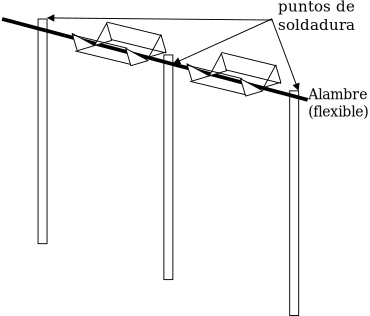
\includegraphics[width=0.4\linewidth]{g02e05}
	\end{center}


\item\label{torsion} Considere un sistema similar al de de la figura con los extremos fijos a \SI{20}{cm} de cada barra.
\begin{enumerate}
	\item Discuta cualitativamente a priori como espera que sean los modos normales, y como serán sus frecuencias comparadas con las del sistema con extremos libres.
	\item Resuelva el problema analíticamente, suponiendo que hay pérdidas proporcionales a la
	      velocidad de torsión que dominan los mecanismos de pérdidas.
		  Discuta como se comparan las resonancias con el caso libre.
	\item Si se fuerza uno de los péndulos de modo que oscile con una amplitud fija a una frecuencia fija, ¿cómo será el movimiento del otro péndulo?
\end{enumerate}
    \begin{center}
		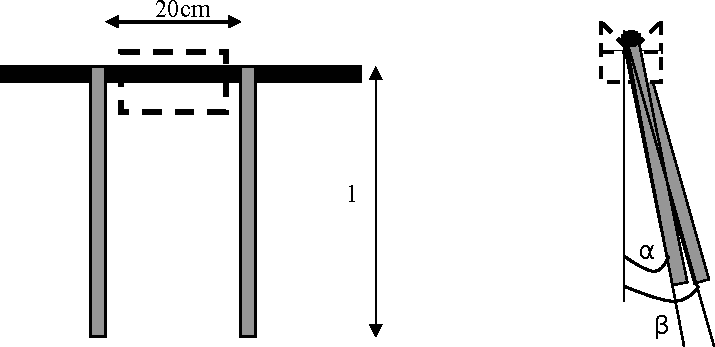
\includegraphics[width=0.4\linewidth]{g02e06}
	\end{center}

\item Dado el sistema de la figura, supuesto en el equilibrio en las condiciones del dibujo, calcule sus frecuencias y modos normales,
	\begin{enumerate}
		\item cuando todos los resortes son slinkies.
		\item cuando las longitudes naturales de los resortes son menores que las graficadas.
	\end{enumerate}
    \begin{center}
		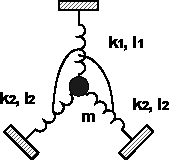
\includegraphics[width=0.25\linewidth]{g02e07}
	\end{center}


\item Encuentre los modos normales de los osciladores acoplados en los dos casos discutidos de acoplamiento ``débil'' y ``fuerte'' y muestre solamente para el caso \(\left| \omega_1^2 - \omega_2^2 \right|\gg \omega_\mathrm{ac}^2 \) que los modos se parecen a los de los osciladores desacoplados.


\item Considere el caso de las barras rígidas acopladas con el resorte de torsión presentado en el ejercicio \ref{torsion} ahora con los extremos libres. Se desea asimetrizar el sistema agregándole una pesa a una de las barras. ¿Cuán grande debe ser esa pesa para que el sistema se lo pueda considerar esencialmente desacoplado.


\item Considere el sistema de dos péndulos de igual longitud \(l\) pero de masas diferentes \(m_a\) y \(m_b\), acoplados mediante un resorte de constante \(k\).
\begin{enumerate}
	\item Escriba las ecuaciones de movimiento de cada masa.
	\item Obtenga las frecuencias naturales del sistema y sus modos normales de oscilación.
		Interprete el significado físico de estos modos normales.
	\item Suponiendo que el acoplamiento es débil y que las condiciones iniciales son \(\Psi_a(0)= 0\) y \(\Psi_b(0)= 1\) y las velocidades iniciales son cero, obtenga el movimiento de cada masa y grafíquelo en función del tiempo.
	\item Calcule los valores medios, en un ciclo rápido, de las siguientes magnitudes \(T_a\), \(T_b\), \(V_a\) y \(V_b\), donde \(T\) indica energía cinética y \(V\) energía potencial gravitatoria.
		Demuestre que bajo la hipótesis de acoplamiento débil \(\langle T_a \rangle \sim \langle V_a \rangle\) (\(\langle \rangle=\)valor medio) y \(\langle T_b \rangle \sim \langle V_b \rangle \).
		Grafique \(\langle E_a \rangle\) y \(\langle E_b \rangle\), y analice las diferencias en el gráfico como función de las diferencias entre las masas (\(m_a=m_b\), y \(m_a\) muy diferente de \(m_b\)).
		Calcule el valor medio de la energía de interacción entre las dos partículas.
	\end{enumerate}
    \begin{center}
		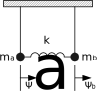
\includegraphics[width=0.25\linewidth]{g02e10}
	\end{center}


\end{enumerate}
\end{document}
